\documentclass[12pt,reqno,oneside]{article}
\usepackage{amsmath}
\usepackage{amssymb}
\usepackage{tikz}
\usetikzlibrary{
  matrix,
  arrows,
  arrows.meta,
  angles,
  shapes,
  backgrounds,
  fit,
  cd,
  calc,
  positioning,
  intersections,
  decorations.markings,
  decorations.pathmorphing,
  backgrounds,patterns,
  decorations.pathreplacing}
\usetikzlibrary{external}
\usepackage{tikz-3dplot}
\usetikzlibrary{decorations.fractals,spy}
\usepackage{xcolor}

\begin{document}

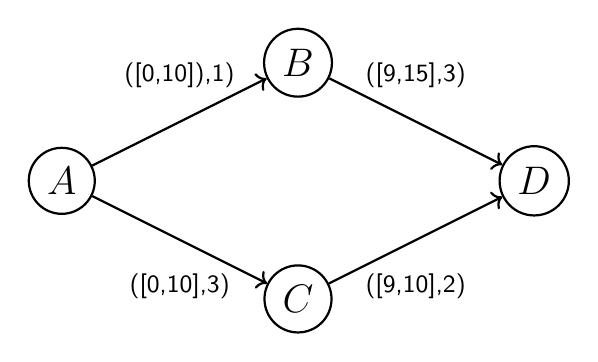
\begin{tikzpicture}[->,auto,node distance=3cm,
      thick,main node/.style={circle,draw,font=\sffamily\Large\bfseries},scale=1.5]
      %Author: Jacob Cleveland
    
      \node[main node] (1) at (-2,0) {$A$};
      \node[main node] (2) at (0,1) {$B$};
      \node[main node] (3) at (0,-1) {$C$};
      \node[main node] (4) at (2,0) {$D$};
    
      \path[every node/.style={font=\sffamily\small}]
          (1) edge[black] node [above=3mm] {([0,10]),1)} (2)
          (1) edge[black] node [below=3mm] {([0,10],3)} (3)
          (2) edge[black] node [above=3mm] {([9,15],3)} (4)
          (3) edge[black] node [below=3mm] {([9,10],2)} (4);
    \end{tikzpicture}

\end{document}